\documentclass[a4paper,12pt]{article}
\usepackage[utf8]{inputenc}
\usepackage{ae}
\usepackage{pslatex}
\usepackage[portuges]{babel}
\usepackage{indentfirst}
\usepackage[portuguese,noprefix]{nomencl}
\usepackage{setspace}
\usepackage[colorlinks,allcolors=black]{hyperref}
\usepackage{enumitem}
\usepackage[ampersand]{easylist}
\usepackage{fancyhdr}
\usepackage{graphicx}

\setlength{\oddsidemargin}{2.5cm}
\setlength{\evensidemargin}{2.5cm}
\setlength{\textwidth}{15cm}
\addtolength{\oddsidemargin}{-1in}
\addtolength{\evensidemargin}{-1in}
\setlength{\topmargin}{2.0cm}
\setlength{\headheight}{1.0cm}
\setlength{\headsep}{1.0cm}
\setlength{\textheight}{22.7cm}
\setlength{\footskip}{1.0cm}
\addtolength{\topmargin}{-1in}
\singlespacing

\begin{document}
\begin{titlepage}
\begin{center}
\centering
\linespread{2.0}
\Huge\Huge\textbf{M1} \\
\huge\huge\textbf{Projeto de modelagem} \\
\LARGE\LARGE\textbf{Sistema de gerenciamento de votos} \\
\vfill
\end{center}
\textbf{Discente: } Ailson Forte dos Santos \\
\textbf{Disciplina: } DIM0504 - Análise de Projeto Orientado a Objetos (APOO) \\
{\par\hfill\today}
\end{titlepage}
\newpage
\tableofcontents

\newpage
\section*{Descrição da aplicação}
\markright{}
\addcontentsline{toc}{section}{Descrição da aplicação}
Desde os tempos mais antigos a humanidade busca conhecer os padrões existentes no mundo. Uma das ferramentas que criamos para esse fim foi a coleta e análise de dados. Os primeiros censos demográficos que se tem notícia foram elaborados pelos chineses e romanos e eram executados por militares e fiscais. O mais antigo é datado de 2238 a.C. realizado na China pelo imperador Yao com o objetivo de coletar informações sobre o número de pessoas e lavouras cultivadas.
\par Dentre as formas de realização de censo, destacamos as pesquisas de opinião, com o intuito de mostrar a realização da democracia. Elas nos mostram como está a satisfação de um determinado grupo de individuos, ou seja, um país, estado, pessoas de uma mesma religião, etc; com relação ao assunto abordado pela pesquisa.
\par Desenvolveremos nesse projeto um sitema que visa gerenciar essas pesquisas. Nosso intuito é, através de enquetes e eleições, falitar a coleta desses dados. Seja para propósitos simples como a cor favorita de determinado grupo de indivíduos ou algo mais complexo como a eleição para presidente de um país. Nela, o usuário poderá criar e gerenciar sua própria pesquisa ou eleição.

\newpage
\section*{Requisitos}
\markright{}
\addcontentsline{toc}{section}{Requisitos}
\subsection*{Regras gerais deste sistema:}
\markright{}
\addcontentsline{toc}{subsection}{Regras gerais deste sistema}

\begin{easylist}[itemize]
& O sistema possui eleitores e juizes de eleição.
& As enquetes/eleições só devem ser cadastradas por juízes de eleição.
& Qualquer usuário não cadastrado é eleitor. Eleitores e juízes de eleição podem votar livremente de acordo com as regras estabelecidas pelo juiz criador da enquete/eleição.
& Juízes de eleição não podem modificar votos, apenas validá-los.
& Todo voto é secreto e direto, ou seja, apenas juízes podem ver quem votou e divulgar o resultado da votação de suas próprias enquetes/eleições.
\end{easylist}

\newpage
\section*{Casos de uso}
\markright{}
\addcontentsline{toc}{section}{Casos de uso}
\subsection*{Diagrama de casos de uso}
\markright{}
\addcontentsline{toc}{subsection}{Diagrama de casos de uso}
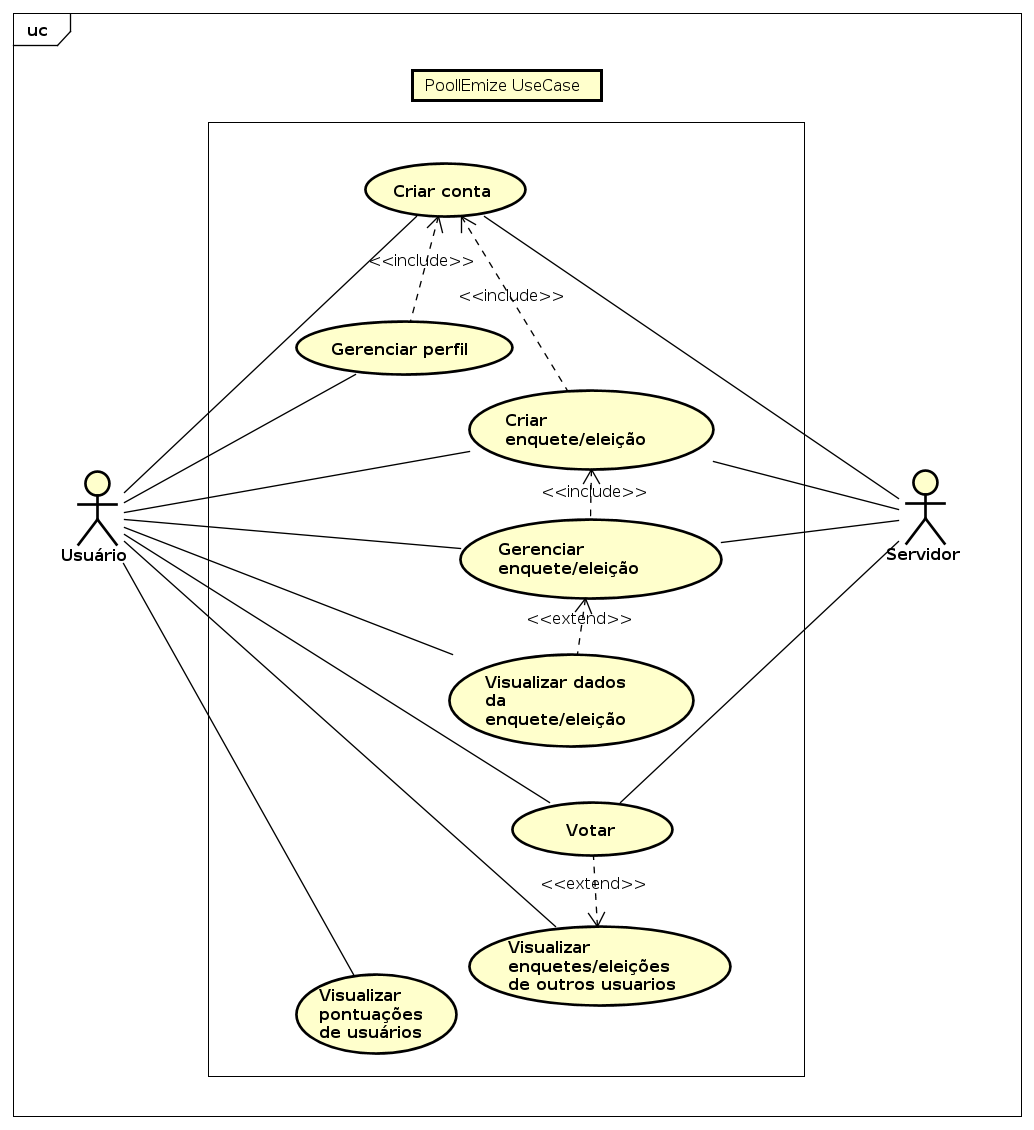
\includegraphics[width=15cm]{use_cases/UseCaseDiagram0.png}
\newpage
\subsection*{Descrição dos casos de uso}
\markright{}
\addcontentsline{toc}{subsection}{Descrição dos casos de uso}

\begin{center}
{\subsubsection*{Criar Conta (CSU01)}}
\end{center}
\markright{}
\addcontentsline{toc}{subsubsection}{Criar Conta (CSU01)}
\begin{tabular}{|l|}\hline
	{\textbf{Sumario:}} Usuário usa o sistema para criar uma conta de juiz eleitoral. \\\\
	{\textbf{Ator primário:}} Usuário \\
	{\textbf{Atores Secundários:}} Servidor\\\\
	{\textbf{Fluxo Principal}}\\
	1. O usuário solicita a realização do cadastro.\\
	2. O usuário é redirecionado para a tela de cadastro. \\
	3. O usuário preenche suas informações, confirma o cadastro e aguarda verificação de email.\\
	4. Após a verificação do cadastro, os dados são enviados ao servidor e o usuário é direcionado\\ a tela principal de enquetes/eleições.\\\\
	{\textbf{Pós-condições:}} O usuário se torna juiz.\\
	\hline
\end{tabular}

\begin{center}
	{\subsubsection*{Gerenciar Perfil(CSU02)}}
\end{center}
\markright{}
\addcontentsline{toc}{subsubsection}{Gerenciar Perfil(CSU02)}
\begin{tabular}{|l|}\hline
	{\textbf{Sumario:}} Usuário usa o sistema para gerenciar suas informações pessoais na conta de juiz\\ eleitoral. \\\\
	{\textbf{Ator primário:}} Usuário \\\\
	{\textbf{Precondições:}} O usuário é juiz.\\\\
	{\textbf{Fluxo Principal}}\\
	1. O usuário solicita ao sistema a visualização dos dados cadastrados.\\
	2. O usuário é redirecionado para a tela de configurações. \\
	3. O usuário visualiza suas informações. \\
	4. Após a verificação dos dados, eles são enviados ao servidor e o usuário é direcionado a tela\\ principal de enquetes/eleições.\\\\
	{\textbf{Fluxo Alternativo(03):}}\\
	a. O usuário atualiza as informações da enquete.\\\\
	{\textbf{Pós-condições:}} O cadastro está atulaizado ou o usuário apenas verificou suas informações.\\
	\hline
\end{tabular}
\\\\
\begin{center}
	{\subsubsection*{Criar Enquete/Eleição(CSU03)}}
\end{center}
\markright{}
\addcontentsline{toc}{subsubsection}{Criar Enquete/Eleição(CSU03)}
\begin{tabular}{|l|}\hline
	{\textbf{Sumario:}} Usuário usa o sistema para gerenciar informações de suas enquetes/eleições.\ \ \ \ \ \ \ \ \ \ \\\\
	{\textbf{Ator primário:}} Usuário \\
	{\textbf{Atores Secundários:}} Servidor\\\\
	{\textbf{Precondições:}} O usuário é juiz.\\\\
	{\textbf{Fluxo Principal}}\\
	1. O usuário solicita ao sistema a visualização das enquetes/eleições.\\
	2. O usuário é redirecionado para a tela de enquetes/eleições. \\
	3. O usuário aperta o botão de criar nova enquete/eleição. \\
	4. O usuário entra com as informações da nova enquete/eleição.\\
	5. O usuário confirma as informações.\\
	6. O usuário altera as consigurações de visualização da enquete/eleição.\\
	7. O usuário salva a enquete/eleição no servidor.\\
	8. O usuário é redirecionado a tela de visualização das enquetes/eleições.\\\\
	{\textbf{Pós-condições:}} As enquetes/eleições do usuário são atualizadas.\\
	\hline
\end{tabular}

\begin{center}
	{\subsubsection*{Gerenciar Enquete/Eleição(CSU04)}}
\end{center}
\markright{}
\addcontentsline{toc}{subsubsection}{Gerenciar Enquete/Eleição(CSU04)}
\begin{tabular}{|l|}\hline
	{\textbf{Sumario:}} Usuário usa o sistema para gerenciar informações de suas enquetes/eleições.\ \ \ \ \ \ \ \ \ \\\\
	{\textbf{Ator primário:}} Usuário \\
	{\textbf{Atores Secundários:}} Servidor\\\\
	{\textbf{Precondições:}} O usuário é juiz. O usuário criou, ao menos uma, enquete/eleição.\\\\
	{\textbf{Fluxo Principal}}\\
	1. O usuário solicita ao sistema a visualização das enquetes/eleições.\\
	2. O usuário é redirecionado para a tela de enquetes/eleições. \\
	3. O usuário seleciona a enquete/eleição que deseja gerenciar. \\
	4. O usuário entra com as novas informações da enquete/eleição.\\
	5. O usuário confirma as informações.\\
	6. O usuário salva a enquete/eleição no servidor.\\
	7. O usuário é redirecionado a tela de visualização das enquetes/eleições.\\\\
	{\textbf{Fluxo Alternativo(04):}}\\
	a. O usuário altera as consigurações de visualização da enquete/eleição.\\\\
	{\textbf{Pós-condições:}} As enquetes/eleições do usuário são atualizadas.\\
	\hline
\end{tabular}
\\\\
\begin{center}
	{\subsubsection*{Visualizar Dados de Enquete/Eleição(CSU05)}}
\end{center}
\markright{}
\addcontentsline{toc}{subsubsection}{Visualizar Dados de Enquete/Eleição(CSU05)}
\begin{tabular}{|l|}\hline
	{\textbf{Sumario:}} Usuário usa o sistema para visualizar informações de suas enquetes/eleições.\ \ \ \ \ \ \ \ \ \\\\
	{\textbf{Ator primário:}} Usuário \\\\
	{\textbf{Precondições:}} O usuário é juiz. O usuário criou, ao menos uma, enquete/eleição.\\\\
	{\textbf{Fluxo Principal}}\\
	1. O usuário solicita ao sistema a visualização das enquetes/eleições.\\
	2. O usuário é redirecionado para a tela de enquetes/eleições. \\
	3. O usuário seleciona a enquete/eleição que deseja visualizar. \\
	4. O usuário solicita ser redirecionado a tela de visualização das enquetes/eleições.\\
	\hline
\end{tabular}

\begin{center}
	{\subsubsection*{Visualizar Enquetes/Eleições de Outros Usuários(CSU06)}}
\end{center}
\markright{}
\addcontentsline{toc}{subsubsection}{Visualizar Enquetes/Eleições de Outros Usuários(CSU06)}
\begin{tabular}{|l|}\hline
	{\textbf{Sumario:}} Usuário usa o sistema para visualizar informações de enquetes/eleições de outros \hfill \\ usuários. \\\\
	{\textbf{Ator primário:}} Usuário \\\\
	{\textbf{Fluxo Principal}}\\
	1. O usuário solicita ao sistema a visualização das enquetes/eleições.\\
	2. O usuário é redirecionado para a tela de enquetes/eleições. \\
	3. O usuário seleciona a enquete/eleição que deseja visualizar. \\
	4. O usuário solicita ser redirecionado a tela de visualização das enquetes/eleições.\\
	\hline
\end{tabular}
\\\\
\begin{center}
	{\subsubsection*{Votar(CSU07)}}
\end{center}
\markright{}
\addcontentsline{toc}{subsubsection}{Votar(CSU07)}
\begin{tabular}{|l|}\hline
	{\textbf{Sumario:}} Usuário usa o sistema para votar em enquetes/eleições de outros usuários.\ \ \ \ \ \ \ \ \ \ \ \ \ \\\\
	{\textbf{Ator primário:}} Usuário \\
	{\textbf{Atores secundários:}} Servidor\\
	{\textbf{Precondições:}} CSU06.\\\\
	{\textbf{Fluxo Principal}}\\
	1. O usuário solicita ao sistema a visualização da enquete/eleição que deseja votar.\\
	2. O usuário seleciona a opção de voto desejada.\\
	3. O usuário seleciona o botão de votar.\\
	4. O sistema salva o voto para a validação do juiz.\\
	5. O usuário recebe a confirmação do voto.\\
	6. O usuário é redirecionado a tela de visualização das enquetes/eleições.\\\\
	{\textbf{Pós-condições:}} O servidor atualiza os dados da enquete/eleição.\\
	\hline
\end{tabular}

\begin{center}
	{\subsubsection*{Visualizar Pontuações de Usuários(CSU08)}}
\end{center}
\markright{}
\addcontentsline{toc}{subsubsection}{Visualizar Pontuações de Usuários(CSU08)}
\begin{tabular}{|l|}\hline
	{\textbf{Sumario:}} Usuário usa o sistema para visualizar pontuações de usuários.\ \ \ \ \ \ \ \ \ \ \ \ \ \ \ \ \ \ \ \ \ \ \ \ \ \ \ \ \ \ \ \ \ \\\\
	{\textbf{Ator primário:}} Usuário \\\\
	{\textbf{Fluxo Principal}}\\
	1. O usuário solicita ao sistema a visualização de pontuação.\\
	2. O usuário é redirecionado para a tela de visualização de pontuação. \\
	3. O usuário seleciona o ranking que deseja visualizar. \\
	4. O usuário solicita ser redirecionado a tela inicial.\\
	\hline
\end{tabular}

\newpage
\section*{Diagrama de Classes de Domínio}
\markright{}
\addcontentsline{toc}{section}{Diagrama de Classes de Domínio}
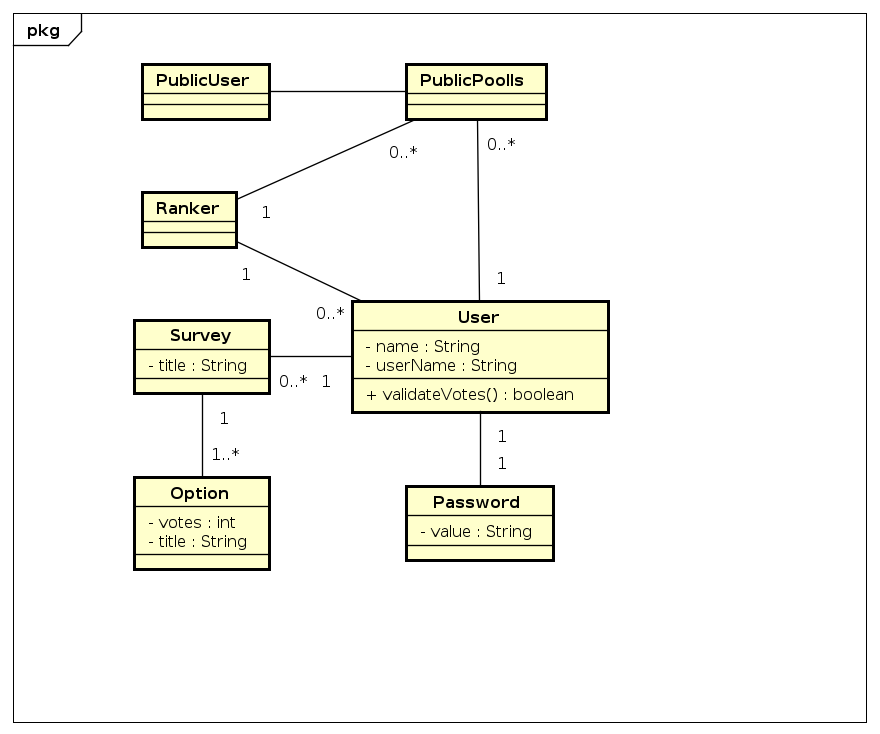
\includegraphics[width=15cm]{class_diagrams/ClassDiagram0.png}

\newpage
\begin{thebibliography}{9}
	\bibitem{bezerra15}
	BEZERRA, E.
	\textit{Princípios de Análise e Projeto de Sistemas com UML.}
	 3. ed. rev. atual.
	 Elsevier/Campus,
	 2015.
	 416 p.
	\bibitem{url1}
	\url{https://www.aedb.br/seget/arquivos/artigos13/28518220.pdf}
	\bibitem{url2}
	\url{https://en.wikipedia.org/wiki/Census}
	\bibitem{url3}
	\url{https://en.wikipedia.org/wiki/Demography}
\end{thebibliography}
\markright{}
\addcontentsline{toc}{section}{Referências}


\end{document}